\chapter{Instalación}

La instalación se llevará por medio de la consola del sistema operativo (Ubuntu), por lo que primero debe acceder a la misma por medio de la combinación de teclas Ctrl + Alt + T.

\begin{figure}[htbp!]
	\begin{center}
		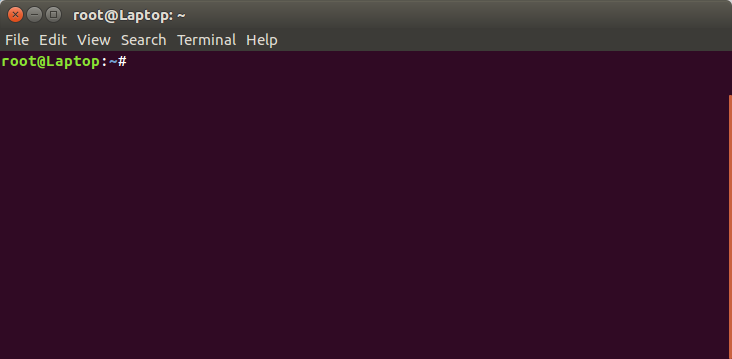
\includegraphics[scale=0.35]{images/INST/1.png}
		\caption{Terminal del sistema.}
	\end{center}
\end{figure}

\section{Instalación PostgreSQL}

\subsection{Purga del sistema}

Al inicio es necesario remover cualquier posible versi\'on que exista en el sistema que pueda entrar en conflicto con la que se intenta instalar, para ello debe ejecutar los siguientes comandos.
\bigbreak
En primer lugar, detiene los posibles servicios relacionados en ejecuci\'on.

\begin{minted}
[
frame=lines,
framesep=2mm,
baselinestretch=1.2,
fontsize=\footnotesize,
linenos
]
{bash}
/etc/init.d/postgresql stop
sudo systemctl stop postgresql.service
\end{minted}

\begin{figure}[htbp!]
	\begin{center}
		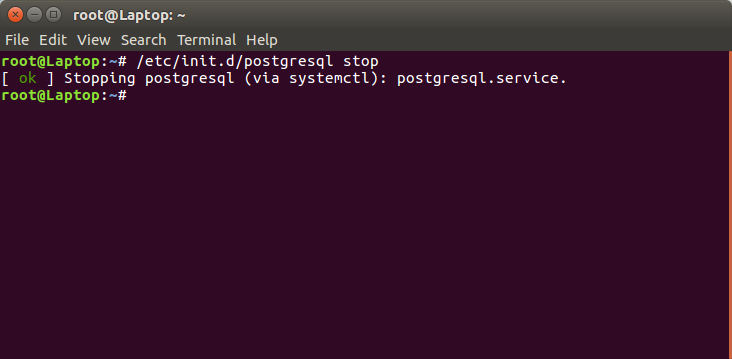
\includegraphics[scale=0.35]{images/INST/2.png}
		\caption{Mensaje de confirmación de la detención del servicio.}
	\end{center}
\end{figure}

\bigbreak
A continuaci\'on, elimina los archivos y ficheros relacionados.

\begin{minted}
[
frame=lines,
framesep=2mm,
baselinestretch=1.2,
fontsize=\footnotesize,
linenos
]
{bash}
sudo apt-get --purge remove postgresql\*
sudo rm -r /etc/postgresql/
sudo rm -r /etc/postgresql-common/
sudo rm -r /var/lib/postgresql/
sudo userdel -r postgres
sudo groupdel postgres
sudo apt-get remove --auto-remove pgadmin4
\end{minted}

\begin{figure}[htbp!]
	\begin{center}
		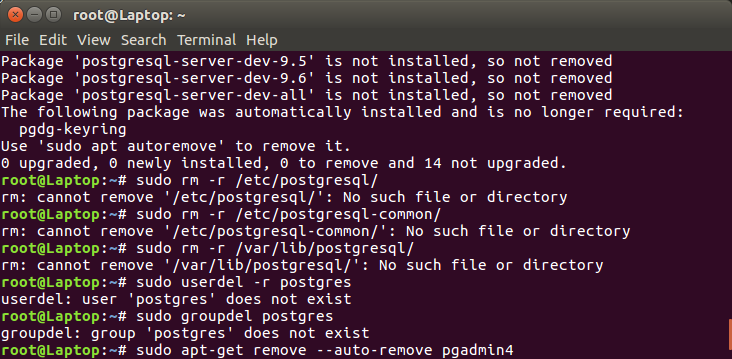
\includegraphics[scale=0.35]{images/INST/3.png}
		\caption{Purga del sistema.}
	\end{center}
\end{figure}

\bigbreak
Procede a descargar e instalar PostgreSQL, as\'i como PGAdmin4 que ser\'a el administrador auxiliar.

\subsection{Instalaci\'on}
\begin{minted}
[
frame=lines,
framesep=2mm,
baselinestretch=1.2,
fontsize=\footnotesize,
linenos
]
{bash}
sudo apt-get update
sudo apt-get install postgresql postgresql-11
sudo apt-get install pgadmin4
\end{minted}

\begin{figure}[htbp!]
	\begin{center}
		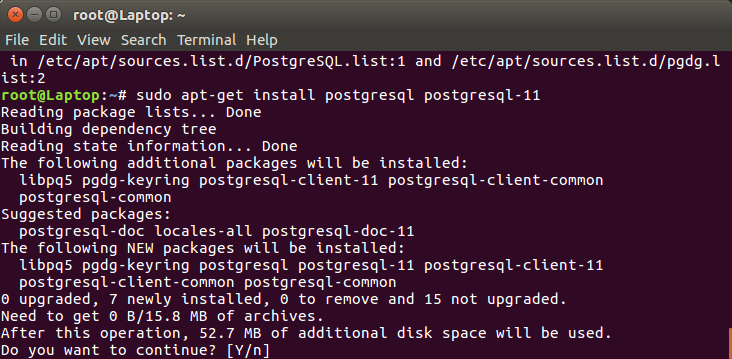
\includegraphics[scale=0.35]{images/INST/4.png}
		\caption{Instalación PostgreSQL.}
	\end{center}
\end{figure}

\bigbreak
\section{Verificación}

Lo siguiente es verificar si se instal\'o correctamente el Adminsitrador de Base de Datos, para ello ejecuta el siguiente comando y debe aparecer la versi\'on instalada previamente.

\subsection{Instalaci\'on PostgreSQL}
\begin{minted}
[
frame=lines,
framesep=2mm,
baselinestretch=1.2,
fontsize=\footnotesize,
linenos
]
{bash}
psql --version
\end{minted}

\begin{figure}[htbp!]
	\begin{center}
		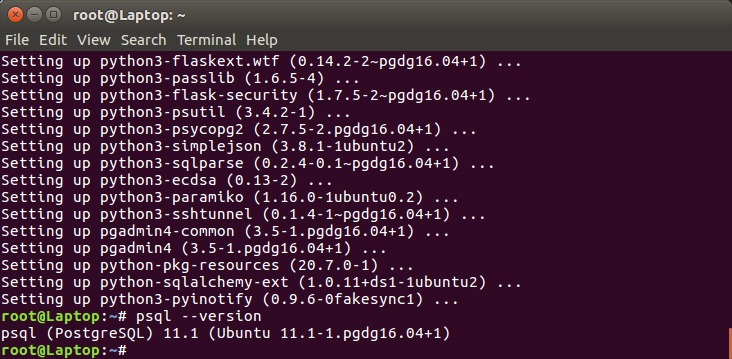
\includegraphics[scale=0.35]{images/INST/5.png}
		\caption{Verificación instalación.}
	\end{center}
\end{figure}

\bigbreak
\section{Configuración del Sistema}

Una vez instalado el Administrador de la Base de Datos, procede a configurar el sistema por medio de la creación de un usuario específico que llevará los procesos relacionados a la Base de Datos para posteriormente incializar la misma.

\subsection{Creaci\'on del usuario}

Añade un usuario tipificado como 'postgres', la contraseña que le colocará será la que se le proporcione al momento de hacerle entrega del sistema.

\begin{minted}
[
frame=lines,
framesep=2mm,
baselinestretch=1.2,
fontsize=\footnotesize,
linenos
]
{bash}
sudo passwd postgres
\end{minted}

\begin{figure}[htbp!]
	\begin{center}
		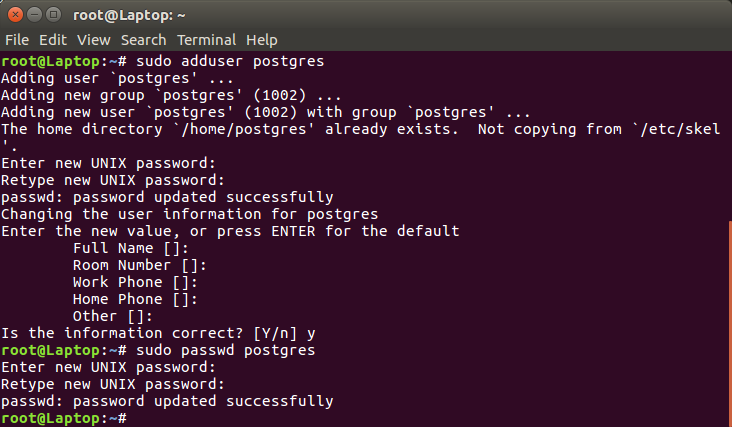
\includegraphics[scale=0.35]{images/INST/6.png}
		\caption{Creación del usuario.}
	\end{center}
\end{figure}

\subsection{Acceso al usuario}

A modo de verificación de lo anterior, así como paso intermedio para los subsecuentes, inicia los servicios del Administrador de la Base de Datos y accede al usuario recién creado.

\begin{minted}
[
frame=lines,
framesep=2mm,
baselinestretch=1.2,
fontsize=\footnotesize,
linenos
]
{bash}
sudo systemctl start postgresql.service
sudo -i -u postgres
\end{minted}

\begin{figure}[htbp!]
	\begin{center}
		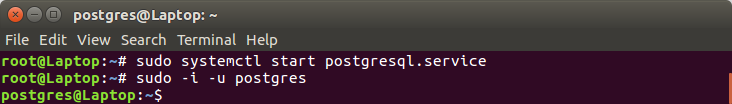
\includegraphics[scale=0.35]{images/INST/7.png}
		\caption{Acceso al usuario.}
	\end{center}
\end{figure}

\subsection{Acceso a PostgreSQL}

Establece los permisos para el perfil Administrador de la Base de Datos.

\begin{minted}
[
frame=lines,
framesep=2mm,
baselinestretch=1.2,
fontsize=\footnotesize,
linenos
]
{bash}
psql
\end{minted}
\begin{minted}
[
frame=lines,
framesep=2mm,
baselinestretch=1.2,
fontsize=\footnotesize,
linenos
]
{postgresql}
ALTER USER postgres PASSWORD 'root';
create database apms;
\c apms
\end{minted}

\begin{figure}[htbp!]
	\begin{center}
		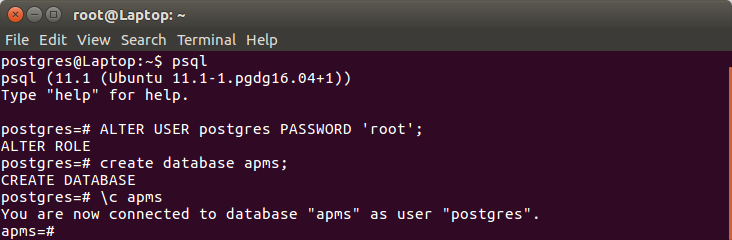
\includegraphics[scale=0.35]{images/INST/8.png}
		\caption{Establecimiento de permisos para la Base de Datos.}
	\end{center}
\end{figure}